\documentclass[11pt]{beamer}
\usetheme{Warsaw}
\usecolortheme{whale}
\usepackage[utf8]{inputenc}
\usepackage[english]{babel}
\usepackage{amsmath}
\usepackage{mathabx}
\usepackage{mathtools}
\usepackage{qtree}
\usepackage{amsfonts}
\usepackage{amssymb}
\usepackage{multimedia}
\author{Joe Duffin}
\title{A Theorem Proving Assistant}
\setbeamercovered{transparent}
\setbeamertemplate{navigation symbols}{}
\titlegraphic{
\includegraphics[width=0.9cm]{logo}}
\institute{School of Computer Science \\University College Dublin}
\date{20th March 2017}
\subject{Final Year Project Presentation}
%\setbeamertemplate{footline}[page number]

\begin{document}

\setlength{\abovedisplayskip}{0pt}
\setlength{\belowdisplayskip}{0pt}
\setlength{\abovedisplayshortskip}{0pt}
\setlength{\belowdisplayshortskip}{0pt}

\begin{frame}
\titlepage
\end{frame}

%\begin{frame}
%\tableofcontents
%\end{frame}

%%%%%%%%%%%%%%%%%%%%%%%%%%%%%%%%%%%%%%%%%%%%%%%%%%%%%%%%%%%%%%%%%%%%
\begin{frame}{Overview}
\begin{itemize}
\setlength\itemsep{2em}
\item \Large{What is Theorem Proving}
\item \Large{What I Built}
\item \Large{How does it work}
\end{itemize}
\end{frame}

%%%%%%%%%%%%%%%%%%%%%%%%%%%%%%%%%%%%%%%%%%%%%%%%%%%%%%%%%%%%%%%%%%%%
\begin{frame}{What is a Theorem?}
\begin{itemize}
\item \Large{A Theorem is a proposition which is not necessarily self-evident but can be proved with a chain of reasoning.}\\
\end{itemize}
\vspace{1cm}
\begin{Theorem}[$\vee zero$]
\large{$P \vee true \equiv true$}
\end{Theorem}
\end{frame}

%%%%%%%%%%%%%%%%%%%%%%%%%%%%%%%%%%%%%%%%%%%%%%%%%%%%%%%%%%%%%%%%%%%%
\begin{frame}{What is Theorem Proving?}

\begin{columns}[c]

\column{.45\textwidth} % Left column and width
\begin{block}{Proof of $\vee zero$}
\begin{align*}
&P \vee true \\
\equiv&\ \ \{(X:\coloneqq P).(0)\} \\
&P \vee ( P \equiv P ) \\
\equiv&\ \ \{(X,Y,Z\coloneqq P,P,P ).(1)\} \\
&P \vee P \equiv P \vee P \\
\equiv&\ \ \{(X \coloneqq P).(2)\} \\
&P \equiv P \\
\equiv&\ \ \{(X \coloneqq P).(0)\} \\
& true
\end{align*}
\end{block}

\column{.5\textwidth} % Right column and width
\begin{block}{Theorems}

$(0) [X \equiv X \equiv true ]$\\
$(1) [X \vee (Y \equiv Z)$\\
\qquad\qquad\qquad$ \equiv X \vee Y \equiv X \vee Z]$\\
$(2) [X \vee X \equiv X]$

\end{block}

\end{columns}

\end{frame}

%%%%%%%%%%%%%%%%%%%%%%%%%%%%%%%%%%%%%%%%%%%%%%%%%%%%%%%%%%%%%%%%%%%%
\begin{frame}{What I Built}
\begin{center}
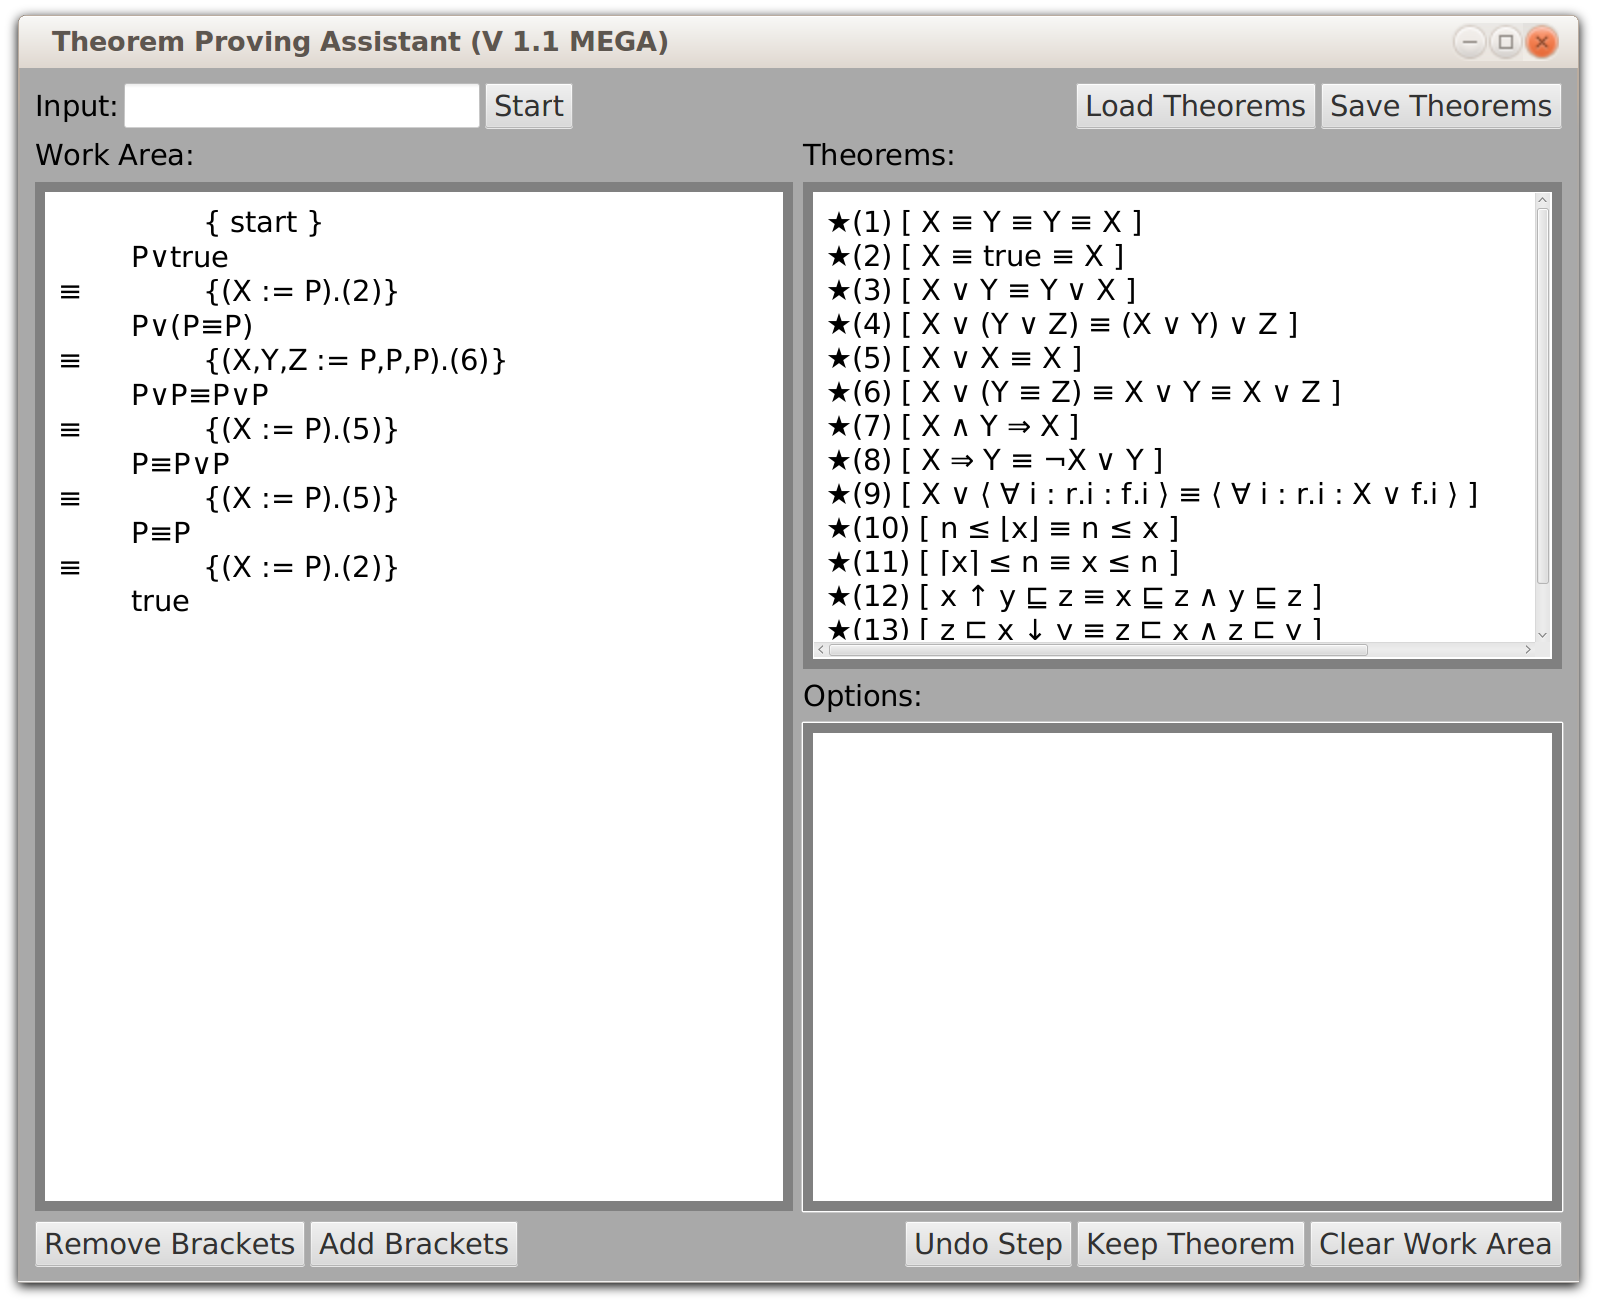
\includegraphics[width=0.9\textwidth]{../TheReport/screenshot}
\end{center}
\end{frame}

%%%%%%%%%%%%%%%%%%%%%%%%%%%%%%%%%%%%%%%%%%%%%%%%%%%%%%%%%%%%%%%%%%%%
\begin{frame}{How it Works - Expression Representation}
\begin{columns}[c]

\column{.45\textwidth} % Left column and width
\begin{block}{String Representation ($Absorbtion0$)}
$X \wedge ( X \vee Y ) \equiv X $
\end{block}
\begin{block}{Tree Representation ($Absorbtion0$)}
\Tree [.$\equiv$ [ X [ [ X Y ].$\vee$ ].$()$ ].$\wedge$ X ]\\
\end{block}

\column{.5\textwidth} % Right column and width
\begin{itemize}
\item \Large{Expressions are represented with syntax trees.}
\end{itemize}
\end{columns}
\end{frame}

%%%%%%%%%%%%%%%%%%%%%%%%%%%%%%%%%%%%%%%%%%%%%%%%%%%%%%%%%%%%%%%%%%%%

\begin{frame}{How it Works - Pattern Matching}

\begin{itemize}
\item \large{Intent: To use the Rule on the User Expression to create a new expression}
\end{itemize}
\vspace{4mm}
\begin{columns}[c]

\column{.45\textwidth} % Left column and width

\begin{block}{Rule (Absorption0)}
$X \wedge ( X \vee Y ) \equiv X $
\end{block}

\column{.5\textwidth} % Right column and width

\begin{block}{User Expression}
$\neg P \wedge ( \neg P \vee Q ) \equiv R \wedge S $
\end{block}

\end{columns}
\vspace{4mm}
\begin{center}
\begin{minipage}{0.5\textwidth}
\begin{block}{New Expression}
$\neg P \equiv R \wedge S $
\end{block}
\end{minipage}
\end{center}


\end{frame}
%%%%%%%%%%%%%%%%%%%%%%%%%%%%%%%%%%%%%%%%%%%%%%%%%%%%%%%%%%%%%%%%%%%%

\begin{frame}{How it Works - Pattern Matching}

\begin{columns}[c]

\column{.45\textwidth} % Left column and width

\begin{block}{Rule:\\$X \wedge ( X \vee Y ) \equiv X $}
\Tree [.$\equiv$ [ X [ [ X Y ].$\vee$ ].$()$ ].$\wedge$  !{\qframesubtree}  \ \ X ]
\end{block}
\begin{block}{Look Up Table}
\ \\
\ 
\end{block}

\column{.5\textwidth} % Right column and width

\begin{block}{User Expression:\\$\neg P \wedge ( \neg P \vee Q ) \equiv R \wedge S $}
\Tree [.$\equiv$  [ [ P ].$\neg$  [ [ [ P ].$\neg$ Q ].$\vee$ ].$()$ ].$\wedge$ !{\qframesubtree} [ \ \ R S ].$\wedge$ ]
\end{block}

\end{columns}

\end{frame}

%%%%%%%%%%%%%%%%%%%%%%%%%%%%%%%%%%%%%%%%%%%%%%%%%%%%%%%%%%%%%%%%%%%%
\begin{frame}{How it Works - Pattern Matching}

\begin{columns}[c]

\column{.45\textwidth} % Left column and width

\begin{block}{Rule:\\$X \wedge ( X \vee Y ) \equiv X $}
\Tree [.$\equiv$ [ X [ [ X Y ].$\vee$ ].$()$ ].\fbox{$\wedge$}  !{\qframesubtree}  \ \ X ]
\end{block}
\begin{block}{Look Up Table}
\ \\
\ 
\end{block}

\column{.5\textwidth} % Right column and width

\begin{block}{User Expression:\\$\neg P \wedge ( \neg P \vee Q ) \equiv R \wedge S $}
\Tree [.$\equiv$  [ [ P ].$\neg$  [ [ [ P ].$\neg$ Q ].$\vee$ ].$()$ ].\fbox{$\wedge$} !{\qframesubtree} [ \ \ R S ].$\wedge$ ]
\end{block}

\end{columns}

\end{frame}

%%%%%%%%%%%%%%%%%%%%%%%%%%%%%%%%%%%%%%%%%%%%%%%%%%%%%%%%%%%%%%%%%%%%

\begin{frame}{How it Works - Pattern Matching}

\begin{columns}[c]

\column{.45\textwidth} % Left column and width

\begin{block}{Rule:\\$X \wedge ( X \vee Y ) \equiv X $}
\Tree [.$\equiv$ [ \fbox{X} [ [ X Y ].$\vee$ ].$()$ ].$\wedge$  !{\qframesubtree}  \ \ X ]
\end{block}
\begin{block}{Look Up Table}
\ \\
\ 
\end{block}

\column{.5\textwidth} % Right column and width

\begin{block}{User Expression:\\$\neg P \wedge ( \neg P \vee Q ) \equiv R \wedge S $}
\Tree [.$\equiv$  [ [ P ].$\neg$ !{\qframesubtree} [ [ [ P ].$\neg$ Q ].$\vee$ ].$()$ ].$\wedge$ !{\qframesubtree} [ \ \ R S ].$\wedge$ ]
\end{block}

\end{columns}

\end{frame}

%%%%%%%%%%%%%%%%%%%%%%%%%%%%%%%%%%%%%%%%%%%%%%%%%%%%%%%%%%%%%%%%%%%%

\begin{frame}{How it Works - Pattern Matching}

\begin{columns}[c]

\column{.45\textwidth} % Left column and width

\begin{block}{Rule:\\$X \wedge ( X \vee Y ) \equiv X $}
\Tree [.$\equiv$ [ \fbox{X} [ [ X Y ].$\vee$ ].$()$ ].$\wedge$  !{\qframesubtree}  \ \ X ]
\end{block}
\begin{block}{Look Up Table}
\fbox{$X \coloneq \neg P$}\\
\ 
\end{block}

\column{.5\textwidth} % Right column and width

\begin{block}{User Expression:\\$\neg P \wedge ( \neg P \vee Q ) \equiv R \wedge S $}
\Tree [.$\equiv$  [ [ P ].$\neg$ !{\qframesubtree} [ [ [ P ].$\neg$ Q ].$\vee$ ].$()$ ].$\wedge$ !{\qframesubtree} [ \ \ R S ].$\wedge$ ]
\end{block}

\end{columns}

\end{frame}


%%%%%%%%%%%%%%%%%%%%%%%%%%%%%%%%%%%%%%%%%%%%%%%%%%%%%%%%%%%%%%%%%%%%

\begin{frame}{How it Works - Pattern Matching}

\begin{columns}[c]

\column{.45\textwidth} % Left column and width

\begin{block}{Rule:\\$X \wedge ( X \vee Y ) \equiv X $}
\Tree [.$\equiv$ [ X [ [ X Y ].$\vee$ ].$()$ ].\fbox{$\wedge$}  !{\qframesubtree}  \ \ X ]
\end{block}
\begin{block}{Look Up Table}
$X \coloneq \neg P$\\
\ 
\end{block}

\column{.5\textwidth} % Right column and width

\begin{block}{User Expression:\\$\neg P \wedge ( \neg P \vee Q ) \equiv R \wedge S $}
\Tree [.$\equiv$  [ [ P ].$\neg$  [ [ [ P ].$\neg$ Q ].$\vee$ ].$()$ ].\fbox{$\wedge$} !{\qframesubtree} [ \ \ R S ].$\wedge$ ]
\end{block}

\end{columns}

\end{frame}

%%%%%%%%%%%%%%%%%%%%%%%%%%%%%%%%%%%%%%%%%%%%%%%%%%%%%%%%%%%%%%%%%%%%

\begin{frame}{How it Works - Pattern Matching}

\begin{columns}[c]

\column{.45\textwidth} % Left column and width

\begin{block}{Rule:\\$X \wedge ( X \vee Y ) \equiv X $}
\Tree [.$\equiv$ [ X [ [ X Y ].$\vee$ ].\fbox{$()$} ].$\wedge$  !{\qframesubtree}  \ \ X ]
\end{block}
\begin{block}{Look Up Table}
$X \coloneq \neg P$\\
\ 
\end{block}

\column{.5\textwidth} % Right column and width

\begin{block}{User Expression:\\$\neg P \wedge ( \neg P \vee Q ) \equiv R \wedge S $}
\Tree [.$\equiv$  [ [ P ].$\neg$  [ [ [ P ].$\neg$ Q ].$\vee$ ].\fbox{$()$} ].$\wedge$ !{\qframesubtree} [ \ \ R S ].$\wedge$ ]
\end{block}

\end{columns}

\end{frame}

%%%%%%%%%%%%%%%%%%%%%%%%%%%%%%%%%%%%%%%%%%%%%%%%%%%%%%%%%%%%%%%%%%%%

\begin{frame}{How it Works - Pattern Matching}

\begin{columns}[c]

\column{.45\textwidth} % Left column and width

\begin{block}{Rule:\\$X \wedge ( X \vee Y ) \equiv X $}
\Tree [.$\equiv$ [ X [ [ X Y ].\fbox{$\vee$} ].$()$ ].$\wedge$  !{\qframesubtree}  \ \ X ]
\end{block}
\begin{block}{Look Up Table}
$X \coloneq \neg P$\\
\ 
\end{block}

\column{.5\textwidth} % Right column and width

\begin{block}{User Expression:\\$\neg P \wedge ( \neg P \vee Q ) \equiv R \wedge S $}
\Tree [.$\equiv$  [ [ P ].$\neg$  [ [ [ P ].$\neg$ Q ].\fbox{$\vee$} ].$()$ ].$\wedge$ !{\qframesubtree} [ \ \ R S ].$\wedge$ ]
\end{block}

\end{columns}

\end{frame}

%%%%%%%%%%%%%%%%%%%%%%%%%%%%%%%%%%%%%%%%%%%%%%%%%%%%%%%%%%%%%%%%%%%%

\begin{frame}{How it Works - Pattern Matching}

\begin{columns}[c]

\column{.45\textwidth} % Left column and width

\begin{block}{Rule:\\$X \wedge ( X \vee Y ) \equiv X $}
\Tree [.$\equiv$ [ X [ [ \fbox{X} Y ].$\vee$ ].$()$ ].$\wedge$  !{\qframesubtree}  \ \ X ]
\end{block}
\begin{block}{Look Up Table}
$X \coloneq \neg P$\\
\ 
\end{block}

\column{.5\textwidth} % Right column and width

\begin{block}{User Expression:\\$\neg P \wedge ( \neg P \vee Q ) \equiv R \wedge S $}
\Tree [.$\equiv$  [ [ P ].$\neg$  [ [ [ P ].$\neg$ !{\qframesubtree} Q ].$\vee$ ].$()$ ].$\wedge$ !{\qframesubtree} [ \ \ R S ].$\wedge$ ]
\end{block}

\end{columns}

\end{frame}

%%%%%%%%%%%%%%%%%%%%%%%%%%%%%%%%%%%%%%%%%%%%%%%%%%%%%%%%%%%%%%%%%%%%

\begin{frame}{How it Works - Pattern Matching}

\begin{columns}[c]

\column{.45\textwidth} % Left column and width

\begin{block}{Rule:\\$X \wedge ( X \vee Y ) \equiv X $}
\Tree [.$\equiv$ [ X [ [ X Y ].\fbox{$\vee$} ].$()$ ].$\wedge$  !{\qframesubtree}  \ \ X ]
\end{block}
\begin{block}{Look Up Table}
$X \coloneq \neg P$\\
\ 
\end{block}

\column{.5\textwidth} % Right column and width

\begin{block}{User Expression:\\$\neg P \wedge ( \neg P \vee Q ) \equiv R \wedge S $}
\Tree [.$\equiv$  [ [ P ].$\neg$  [ [ [ P ].$\neg$ Q ].\fbox{$\vee$} ].$()$ ].$\wedge$ !{\qframesubtree} [ \ \ R S ].$\wedge$ ]
\end{block}

\end{columns}

\end{frame}

%%%%%%%%%%%%%%%%%%%%%%%%%%%%%%%%%%%%%%%%%%%%%%%%%%%%%%%%%%%%%%%%%%%%

\begin{frame}{How it Works - Pattern Matching}

\begin{columns}[c]

\column{.45\textwidth} % Left column and width

\begin{block}{Rule:\\$X \wedge ( X \vee Y ) \equiv X $}
\Tree [.$\equiv$ [ X [ [ X \fbox{Y} ].$\vee$ ].$()$ ].$\wedge$  !{\qframesubtree}  \ \ X ]
\end{block}
\begin{block}{Look Up Table}
$X \coloneq \neg P$\\
\ 
\end{block}

\column{.5\textwidth} % Right column and width

\begin{block}{User Expression:\\$\neg P \wedge ( \neg P \vee Q ) \equiv R \wedge S $}
\Tree [.$\equiv$  [ [ P ].$\neg$  [ [ [ P ].$\neg$ \fbox{Q} ].$\vee$ ].$()$ ].$\wedge$ !{\qframesubtree} [ \ \ R S ].$\wedge$ ]
\end{block}

\end{columns}

\end{frame}

%%%%%%%%%%%%%%%%%%%%%%%%%%%%%%%%%%%%%%%%%%%%%%%%%%%%%%%%%%%%%%%%%%%%

\begin{frame}{How it Works - Pattern Matching}

\begin{columns}[c]

\column{.45\textwidth} % Left column and width

\begin{block}{Rule:\\$X \wedge ( X \vee Y ) \equiv X $}
\Tree [.$\equiv$ [ X [ [ X \fbox{Y} ].$\vee$ ].$()$ ].$\wedge$  !{\qframesubtree}  \ \ X ]
\end{block}
\begin{block}{Look Up Table}
$X \coloneq \neg P$\\
\fbox{$Y \coloneq Q$}
\end{block}

\column{.5\textwidth} % Right column and width

\begin{block}{User Expression:\\$\neg P \wedge ( \neg P \vee Q ) \equiv R \wedge S $}
\Tree [.$\equiv$  [ [ P ].$\neg$  [ [ [ P ].$\neg$ \fbox{Q} ].$\vee$ ].$()$ ].$\wedge$ !{\qframesubtree} [ \ \ R S ].$\wedge$ ]
\end{block}

\end{columns}

\end{frame}

%%%%%%%%%%%%%%%%%%%%%%%%%%%%%%%%%%%%%%%%%%%%%%%%%%%%%%%%%%%%%%%%%%%%

\begin{frame}{How it Works - Pattern Matching}

\begin{columns}[c]

\column{.45\textwidth} % Left column and width

\begin{block}{Rule:\\$X \wedge ( X \vee Y ) \equiv X $}
\Tree [.$\equiv$ [ X [ [ X Y ].\fbox{$\vee$} ].$()$ ].$\wedge$  !{\qframesubtree}  \ \ X ]
\end{block}
\begin{block}{Look Up Table}
$X \coloneq \neg P$\\
$Y \coloneq Q$
\end{block}

\column{.5\textwidth} % Right column and width

\begin{block}{User Expression:\\$\neg P \wedge ( \neg P \vee Q ) \equiv R \wedge S $}
\Tree [.$\equiv$  [ [ P ].$\neg$  [ [ [ P ].$\neg$ Q ].\fbox{$\vee$} ].$()$ ].$\wedge$ !{\qframesubtree} [ \ \ R S ].$\wedge$ ]
\end{block}

\end{columns}

\end{frame}

%%%%%%%%%%%%%%%%%%%%%%%%%%%%%%%%%%%%%%%%%%%%%%%%%%%%%%%%%%%%%%%%%%%%

\begin{frame}{How it Works - Pattern Matching}

\begin{columns}[c]

\column{.45\textwidth} % Left column and width

\begin{block}{Rule:\\$X \wedge ( X \vee Y ) \equiv X $}
\Tree [.$\equiv$ [ X [ [ X Y ].$\vee$ ].\fbox{$()$} ].$\wedge$  !{\qframesubtree}  \ \ X ]
\end{block}
\begin{block}{Look Up Table}
$X \coloneq \neg P$\\
$Y \coloneq Q$
\end{block}

\column{.5\textwidth} % Right column and width

\begin{block}{User Expression:\\$\neg P \wedge ( \neg P \vee Q ) \equiv R \wedge S $}
\Tree [.$\equiv$  [ [ P ].$\neg$  [ [ [ P ].$\neg$ Q ].$\vee$ ].\fbox{$()$} ].$\wedge$ !{\qframesubtree} [ \ \ R S ].$\wedge$ ]
\end{block}

\end{columns}

\end{frame}

%%%%%%%%%%%%%%%%%%%%%%%%%%%%%%%%%%%%%%%%%%%%%%%%%%%%%%%%%%%%%%%%%%%%

\begin{frame}{How it Works - Pattern Matching}

\begin{columns}[c]

\column{.45\textwidth} % Left column and width

\begin{block}{Rule:\\$X \wedge ( X \vee Y ) \equiv X $}
\Tree [.$\equiv$ [ X [ [ X Y ].$\vee$ ].$()$ ].\fbox{$\wedge$}  !{\qframesubtree}  \ \ X ]
\end{block}
\begin{block}{Look Up Table}
$X \coloneq \neg P$\\
$Y \coloneq Q$
\end{block}

\column{.5\textwidth} % Right column and width

\begin{block}{User Expression:\\$\neg P \wedge ( \neg P \vee Q ) \equiv R \wedge S $}
\Tree [.$\equiv$  [ [ P ].$\neg$  [ [ [ P ].$\neg$ Q ].$\vee$ ].$()$ ].\fbox{$\wedge$} !{\qframesubtree} [ \ \ R S ].$\wedge$ ]
\end{block}

\end{columns}

\end{frame}

%%%%%%%%%%%%%%%%%%%%%%%%%%%%%%%%%%%%%%%%%%%%%%%%%%%%%%%%%%%%%%%%%%%%

\begin{frame}{How it Works - Pattern Matching}

\begin{columns}[c]

\column{.45\textwidth} % Left column and width

\begin{block}{Rule:\\$X \wedge ( X \vee Y ) \equiv X $}
\Tree [.$\equiv$ [ X [ [ X Y ].$\vee$ ].$()$ ].$\wedge$  !{\qframesubtree}  \ \ X ]
\end{block}
\begin{block}{Look Up Table}
$X \coloneq \neg P$\\
$Y \coloneq Q$
\end{block}

\column{.5\textwidth} % Right column and width

\begin{block}{User Expression:\\$\neg P \wedge ( \neg P \vee Q ) \equiv R \wedge S $}
\Tree [.$\equiv$  [ [ P ].$\neg$  [ [ [ P ].$\neg$ Q ].$\vee$ ].$()$ ].$\wedge$ !{\qframesubtree} [ \ \ R S ].$\wedge$ ]
\end{block}

\end{columns}

\end{frame}

%%%%%%%%%%%%%%%%%%%%%%%%%%%%%%%%%%%%%%%%%%%%%%%%%%%%%%%%%%%%%%%%%%%%

\begin{frame}{How it Works - Pattern Matching}

\begin{columns}[c]

\column{.45\textwidth} % Left column and width

\begin{block}{Rule:\\$X \wedge ( X \vee Y ) \equiv X $}
\Tree [.$\equiv$ [ X [ [ X Y ].$\vee$ ].$()$ ].$\wedge$ X !{\qframesubtree}  ]
\end{block}
\begin{block}{Look Up Table}
$X \coloneq \neg P$\\
$Y \coloneq Q$
\end{block}

\column{.5\textwidth} % Right column and width

\begin{block}{User Expression:\\$\neg P \wedge ( \neg P \vee Q ) \equiv R \wedge S $}
\Tree [.$\equiv$  [ [ P ].$\neg$  [ [ [ P ].$\neg$ Q ].$\vee$ ].$()$ ].$\wedge$ !{\qframesubtree} [ \ \ R S ].$\wedge$ ]
\end{block}

\end{columns}

\end{frame}

%%%%%%%%%%%%%%%%%%%%%%%%%%%%%%%%%%%%%%%%%%%%%%%%%%%%%%%%%%%%%%%%%%%%

\begin{frame}{How it Works - Pattern Matching}

\begin{columns}[c]

\column{.45\textwidth} % Left column and width

\begin{block}{Rule:\\$X \wedge ( X \vee Y ) \equiv X $}
\Tree [.$\equiv$ [ X [ [ X Y ].$\vee$ ].$()$ ].$\wedge$ X !{\qframesubtree}  ]
\end{block}
\begin{block}{Look Up Table}
\fbox{$X \coloneq \neg P$}\\
$Y \coloneq Q$
\end{block}

\column{.5\textwidth} % Right column and width

\begin{block}{User Expression:\\$\neg P \wedge ( \neg P \vee Q ) \equiv R \wedge S $}
\Tree [.$\equiv$  [ [ P ].$\neg$  [ [ [ P ].$\neg$ Q ].$\vee$ ].$()$ ].$\wedge$ !{\qframesubtree} [ \ \ R S ].$\wedge$ ]
\end{block}

\end{columns}

\end{frame}


%%%%%%%%%%%%%%%%%%%%%%%%%%%%%%%%%%%%%%%%%%%%%%%%%%%%%%%%%%%%%%%%%%%%

\begin{frame}{How it Works - Pattern Matching}

\begin{columns}[c]

\column{.45\textwidth} % Left column and width

\begin{block}{Rule:\\$X \wedge ( X \vee Y ) \equiv X $}
\Tree [.$\equiv$ [ X [ [ X Y ].$\vee$ ].$()$ ].$\wedge$ [ P ].$\neg$ !{\qframesubtree}  ]
\end{block}
\begin{block}{Look Up Table}
\fbox{$X \coloneq \neg P$}\\
$Y \coloneq Q$
\end{block}

\column{.5\textwidth} % Right column and width

\begin{block}{User Expression:\\$\neg P \wedge ( \neg P \vee Q ) \equiv R \wedge S $}
\Tree [.$\equiv$  [ [ P ].$\neg$  [ [ [ P ].$\neg$ Q ].$\vee$ ].$()$ ].$\wedge$ !{\qframesubtree} [ \ \ R S ].$\wedge$ ]
\end{block}

\end{columns}

\end{frame}

%%%%%%%%%%%%%%%%%%%%%%%%%%%%%%%%%%%%%%%%%%%%%%%%%%%%%%%%%%%%%%%%%%%%

\begin{frame}{How it Works - Pattern Matching}

\begin{columns}[c]

\column{.45\textwidth} % Left column and width

\begin{block}{Rule:\\$X \wedge ( X \vee Y ) \equiv X $}
\Tree [.$\equiv$ [ X [ [ X Y ].$\vee$ ].$()$ ].$\wedge$ [ P ].$\neg$ !{\qframesubtree}  ]
\end{block}
\begin{block}{Look Up Table}
$X \coloneq \neg P$\\
$Y \coloneq Q$
\end{block}

\column{.5\textwidth} % Right column and width

\begin{block}{User Expression:\\$\neg P \equiv R \wedge S $}
\Tree [.$\equiv$ [ P ].$\neg$ !{\qframesubtree} [ \ \ R S ].$\wedge$ ]
\end{block}

\end{columns}

\end{frame}

%%%%%%%%%%%%%%%%%%%%%%%%%%%%%%%%%%%%%%%%%%%%%%%%%%%%%%%%%%%%%%%%%%%%


\begin{frame}{How it Works - Pattern Matching}

\begin{columns}[c]

\column{.45\textwidth} % Left column and width
\begin{block}{Previous Expression}
$\neg P \wedge ( \neg P \vee Q ) \equiv R \wedge S $
\end{block}
\begin{block}{Look Up Table}
$X \coloneq \neg P$\\
$Y \coloneq Q$
\end{block}
\begin{block}{New Expression}
$\neg P \equiv R \wedge S $
\end{block}

\column{.5\textwidth} % Right column and width

\begin{itemize}
\item \large{The new user expression and lookup table are used to generate the hint and next line of the proof.}
\end{itemize}
\begin{block}{The Step}
\begin{align*}
&\neg P \wedge ( \neg P \vee Q ) \equiv R \wedge S \\
\equiv&\qquad\{(X, Y :\coloneqq \neg P, Q ).Abs0\} \\
&\neg P \equiv R \wedge S 
\end{align*}
\end{block}

\end{columns}

\end{frame}

%%%%%%%%%%%%%%%%%%%%%%%%%%%%%%%%%%%%%%%%%%%%%%%%%%%%%%%%%%%%%%%%%%%%

\begin{frame}{Versatility - Supported Calculi}
\begin{itemize}
\setlength\itemsep{2em}
\item \Large{Boolean}
\item \Large{Floor/Ceiling}
\item \Large{Max/Min}
\item \Large{Lattice Theory}
\item \Large{Quantified Notation}
\end{itemize}
\end{frame}

%%%%%%%%%%%%%%%%%%%%%%%%%%%%%%%%%%%%%%%%%%%%%%%%%%%%%%%%%%%%%%%%%%%%
\begin{frame}
\Huge{\centerline{Questions...}}
\end{frame}
\end{document}